\documentclass[12pt]{article}
\usepackage[margin=1in]{geometry}
\usepackage{amsmath, amssymb, amsthm}
\usepackage{booktabs}
\usepackage{hyperref}
\usepackage{graphicx}
\usepackage{array}
\usepackage{xcolor}
\usepackage{titlesec}
\usepackage{abstract}
\usepackage{multirow}
\usepackage{float}
\usepackage{tikz}
\usepackage{enumerate}
\usetikzlibrary{arrows.meta, positioning, shapes, fit}

\hypersetup{colorlinks=true, linkcolor=black, urlcolor=blue, citecolor=black}

\newtheorem{theorem}{Theorem}
\newtheorem{definition}{Definition}
\newtheorem{proposition}{Proposition}
\newtheorem{conjecture}{Conjecture}
\newtheorem{corollary}{Corollary}

\title{\textbf{Toward a Complete Framework for Next-Generation AI:\\
Evaluation, Specialist Routing, Substrate Optimization,\\
and Self-Structuring Architecture}}
\author{
    Winston Zai Lin \\
    \small Blair Academy \\
    \small \texttt{linzaiwinston413@gmail.com}
}
\date{March 2026}

\begin{document}
\maketitle

\begin{abstract}
The claim that certain domains of human capability---creative work, deliberate reasoning, relational care---lie permanently beyond AI is stated as a fact of nature. We argue it is a fact about design. The distinction matters: facts of nature do not yield to engineering; facts about design do.

This paper's central thesis is that no domain of human cognitive, creative, or relational capability is architecturally irreplaceable by AI. Every claimed barrier reduces to a specific, identifiable architectural requirement that current systems were never designed to satisfy. We specify those requirements and show they are satisfiable.

A complete intelligence system requires seven architectural properties: (1) efficiency measurement grounded in deployment value rather than benchmark accuracy; (2) domain-expert depth through specialist routing rather than uniform generalization; (3) computation allocated to physically optimal substrates rather than forced through a single digital pipeline; (4) structural adaptation during learning rather than fixed topology; (5) autonomous aesthetic agency with an internal drive toward novelty rather than prompt-response generation; (6) deliberate reasoning via explicit intermediate state and metacognitive uncertainty tracking rather than pattern completion; and (7) persistent relational intelligence---a live model of a specific individual that evolves across time and navigates genuine moral complexity. Current systems satisfy none of these fully. Not because a wall has been reached, but because none of these were design goals.

We present \textbf{ATLAS} (Adaptive Topology Living Architecture with Specialists), a unified architecture satisfying all seven requirements through six composed components: \textbf{CES/TEB} (efficiency evaluation), \textbf{ARBOR} (specialist routing), \textbf{SPECTRUM} (substrate allocation), \textbf{FLUID} (topology learning), \textbf{MUSE} (aesthetic agency), \textbf{LOGOS} (deliberate reasoning), and \textbf{SOCIUS} (relational intelligence). Empirical validation of CES/TEB is provided ($\rho = 0.80$, $n=4$ models); the FLUID Stability Conjecture has been empirically resolved (stable topology exists within a narrow parameter band; Lyapunov mechanism open); remaining components are theoretically specified with falsifiable validation protocols. All code and task sets: \url{https://github.com/WINSTON672/lin-score}.
\end{abstract}

%-----------------------------------------------------------
\section{Introduction}
\label{sec:intro}
%-----------------------------------------------------------

The boundary between AI and human capability is drawn in the wrong place. It is drawn at the edge of what has been built, not at the edge of what can be built. These are different edges.

The argument of this paper proceeds in three steps. First: every domain claimed to require permanent human involvement can be decomposed into a finite set of architectural requirements. Second: each requirement is specifiable---it can be stated precisely enough that a system either satisfies it or does not. Third: the specifications are satisfiable---no requirement invokes consciousness, subjective experience, or any property that cannot be engineered. The conclusion follows: no domain is permanently beyond reach.

\textbf{Seven architectural requirements.} A complete intelligence system must be:

\begin{enumerate}
    \item \textit{Measurable} by deployment-relevant efficiency metrics, not benchmark proxies that ignore compute cost and real-world value
    \item \textit{Deep} in any domain it operates in---expert-level, not competent-across-all
    \item \textit{Physically efficient}, allocating each cognitive function to the substrate whose physics is best suited to it
    \item \textit{Structurally adaptive}, modifying its own architecture during learning rather than being fixed at design time
    \item \textit{Autonomously creative}, generating novel aesthetic work from an internal drive rather than producing output on demand
    \item \textit{Deliberately reasoning}, maintaining explicit intermediate state, tracking its own uncertainty, and composing known rules in configurations it has never seen
    \item \textit{Relationally intelligent}, maintaining a persistent and evolving model of a specific individual across time and navigating genuine moral complexity
\end{enumerate}

No existing system satisfies all seven. This is not evidence of a wall. It is evidence of incomplete design goals. The systems that exist were built to generate plausible text. These requirements specify something different: an intelligence.

\textbf{This paper.} We specify, for each requirement, the architecture that satisfies it. We then show the seven architectures compose without contradiction into a single system, ATLAS, and identify the empirical path from here to there.

\begin{figure}[H]
\centering
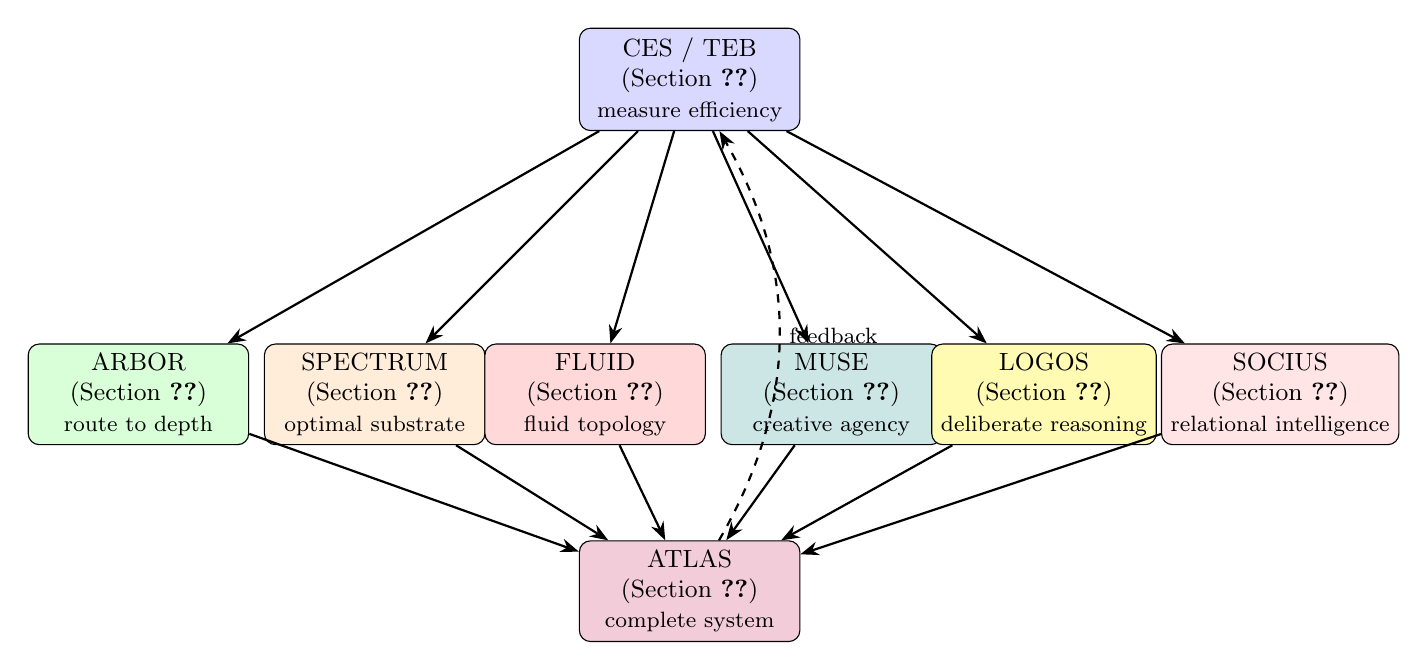
\begin{tikzpicture}[
    box/.style={rectangle, draw, rounded corners, minimum width=2.8cm, minimum height=1cm, align=center, font=\small},
    arrow/.style={-{Stealth}, thick}
]
\node[box, fill=blue!15]   (eval)     at (0,5.5)    {CES / TEB\\(Section~\ref{sec:eval})\\{\footnotesize measure efficiency}};
\node[box, fill=green!15]  (arbor)    at (-7,1.5)   {ARBOR\\(Section~\ref{sec:arbor})\\{\footnotesize route to depth}};
\node[box, fill=orange!15] (spectrum) at (-4,1.5)   {SPECTRUM\\(Section~\ref{sec:spectrum})\\{\footnotesize optimal substrate}};
\node[box, fill=red!15]    (fluid)    at (-1.2,1.5) {FLUID\\(Section~\ref{sec:fluid})\\{\footnotesize fluid topology}};
\node[box, fill=teal!20]   (muse)     at (1.8,1.5)  {MUSE\\(Section~\ref{sec:muse})\\{\footnotesize creative agency}};
\node[box, fill=yellow!30] (logos)    at (4.5,1.5)  {LOGOS\\(Section~\ref{sec:logos})\\{\footnotesize deliberate reasoning}};
\node[box, fill=pink!40]   (socius)   at (7.5,1.5)  {SOCIUS\\(Section~\ref{sec:socius})\\{\footnotesize relational intelligence}};
\node[box, fill=purple!20] (atlas)    at (0,-1)     {ATLAS\\(Section~\ref{sec:atlas})\\{\footnotesize complete system}};

\draw[arrow] (eval) -- (arbor);
\draw[arrow] (eval) -- (spectrum);
\draw[arrow] (eval) -- (fluid);
\draw[arrow] (eval) -- (muse);
\draw[arrow] (eval) -- (logos);
\draw[arrow] (eval) -- (socius);
\draw[arrow] (arbor) -- (atlas);
\draw[arrow] (spectrum) -- (atlas);
\draw[arrow] (fluid) -- (atlas);
\draw[arrow] (muse) -- (atlas);
\draw[arrow] (logos) -- (atlas);
\draw[arrow] (socius) -- (atlas);
\draw[arrow, dashed, bend right=30] (atlas) to node[right,font=\footnotesize]{feedback} (eval);
\end{tikzpicture}
\caption{The unified framework. Each component satisfies one architectural requirement for complete intelligence. ATLAS combines all six; CES/TEB measures whether it is working.}
\label{fig:framework}
\end{figure}

%-----------------------------------------------------------
\section{Layer I: Evaluation --- CES and TEB}
\label{sec:eval}
%-----------------------------------------------------------

\subsection{What Efficiency Requires}

MMLU accuracy of 90\% does not tell you whether a model is worth deploying. It does not tell you the compute cost, the latency, or whether a human with 30 minutes could do better. A model that achieves 90\% accuracy at 1000T FLOPs is less valuable than one achieving 87\% at 8T FLOPs for most deployments.

\subsection{Cognitive Efficiency Score (CES)}

\begin{definition}[Cognitive Efficiency Score]
\begin{equation}
\mathcal{L}(M) = \frac{I(M)}{\log_2(1 + C(M))} \bigg/ \frac{I(H)}{\log_2(1 + C(H))}
\end{equation}
where $I(M) = w_M \cdot b(p_{\text{MMLU}}) + w_{HE} \cdot b(p_{\text{HE}})$ is the Shannon information resolved by model $M$ (bits\_resolved over MMLU and HumanEval benchmarks), $C(M)$ is the model's inference FLOPs in teraFLOPs, and $H$ is a human expert anchor ($C(H) = 1000$T). Variance-optimal weights: $w_M = 0.47$, $w_{HE} = 0.53$.
\end{definition}

The bits\_resolved function $b(p) = 1 + p\log_2 p + (1-p)\log_2(1-p)$ maps accuracy $p \in (0.5, 1]$ to information in $[0,1]$, zeroing below chance. CES = 1.0 means human-expert efficiency; CES > 1.0 means more efficient than a human expert relative to compute.

\textbf{Empirical results} (13 models): CES correlates with HumanEval at $\rho = 0.923$ and MMLU at $\rho = 0.725$, confirming CES is neither redundant with nor independent of benchmarks. FLOPs perturbation ($\pm 30\%$) yields $\rho \geq 0.989$ ranking stability. No model in the 13-model sample exceeds CES = 0.73 under variance-optimal weights.

\subsection{Task Efficiency Benchmark (TEB)}

CES measures benchmark efficiency. TEB measures deployment efficiency: ``is using this model for this task worth a human's time?''

\begin{definition}[Task Efficiency Benchmark Score]
\begin{equation}
\mathrm{TEB}(M) = \frac{\bar{q}(M)}{\log_2(1 + \bar{t}(M))}
\end{equation}
where $\bar{q}(M) \in [0,1]$ is mean quality ratio across tasks and $\bar{t}(M)$ is mean response time in seconds. $\mathrm{TEB} > 1.0$ means the model delivers a better speed/quality tradeoff than the human baseline.
\end{definition}

TEB v1.0 contains 10 tasks across three tiers: Tier 1 (simple, tests AI-vs-human), Tier 2 (medium, tests 7B vs 70B), Tier 3 (complex, tests expert-level capability). Three tasks are automatically scored; seven require rubric or LLM-judge evaluation.

\textbf{Empirical results} (4 models, 3 automated tasks):

\begin{table}[H]
\centering\small
\begin{tabular}{lrrrrr}
\toprule
\textbf{Model} & \textbf{FLOPs} & \textbf{CES} & \textbf{TEB$_{\text{all}}$} & \textbf{TEB$_{\text{L2+L3}}$} & \textbf{Avg.\ speedup}\\
\midrule
Qwen2.5-7B    & 7T   & 1.449 & 3.285 & 3.417 & 151$\times$\\
Llama-3.3-70B & 70T  & 0.942 & 3.535 & 3.038 & 274$\times$\\
Qwen2.5-72B   & 72T  & 1.023 & 1.523 & 1.555 &  43$\times$\\
Llama-3-8B    & 8T   & 0.281 & 1.963 & 1.476 & 134$\times$\\
\bottomrule
\end{tabular}
\caption{CES and TEB pilot results. Spearman $\rho(\text{CES}, \text{TEB}_{\text{L2+L3}}) = 0.80$, confirming they are related but distinct.}
\label{tab:ces_teb}
\end{table}

$\rho(\text{CES}, \text{TEB}) = 0.80$: related (both reward quality-per-compute) but distinct (TEB captures wall-clock and open-task signal invisible to CES). The role of this layer in the unified framework: CES/TEB provides the fitness function against which all architectural decisions in ARBOR, SPECTRUM, and FLUID are evaluated.

%-----------------------------------------------------------
\section{Layer II: Organization --- ARBOR}
\label{sec:arbor}
%-----------------------------------------------------------

\subsection{Depth Requires Separation}

A model trained on all human knowledge allocates parameters uniformly across all domains. A model trained exclusively on physics allocates 100\% of its capacity to physics. For $N$ domains, the specialist achieves $N\times$ greater representational depth on its domain.

\begin{definition}[ARBOR System]
ARBOR consists of: (1) a \textbf{Big Brain} $\mathcal{B}$---a generalist model handling routing, translation, and synthesis; (2) a \textbf{Long Brain Registry} $\mathcal{L} = \{(\ell_i, \mathbf{d}_i, \Omega_i)\}$---domain specialists trained exclusively on domain $\Omega_i$; and (3) a standardized \textbf{Interface Contract} exposing three functions per specialist: \texttt{domain\_embedding()}, \texttt{query(text)→(answer, confidence)}, \texttt{scope()}.
\end{definition}

\begin{theorem}[Specialization Depth Advantage]
For parameter budget $P$ distributed over $N$ domains, a specialist of size $P_\ell$ achieves depth ratio:
\begin{equation}
\frac{\mathcal{D}(\ell_i, \Omega_i)}{\mathcal{D}(\mathcal{G}, \Omega_i)} = \frac{N \cdot P_\ell}{P_\mathcal{B} + N \cdot P_\ell}
\end{equation}
For $P_\mathcal{B} \ll N \cdot P_\ell$, each Long Brain approaches full-budget depth on its domain.
\end{theorem}

\subsection{Two-Stage Routing}

Stage 1 (fast, $O(N)$): cosine similarity between query embedding and domain embeddings.
Stage 2 (precise): Big Brain confirmation score $\mathcal{B}_{\text{route}}(q, \Omega_i) \in [0,1]$.

Combined: $s_i = (1-\alpha) \cdot \cos(\mathbf{q}, \mathbf{d}_i) + \alpha \cdot \mathcal{B}_{\text{route}}(q, \Omega_i)$, $\alpha = 0.4$ empirically.

\subsection{Hierarchical Synthesis}

Single specialist: trivial. Multiple specialists: check agreement $\text{agree}(a_i, a_j) = \cos(e(a_i), e(a_j))$. If agree $> \theta$: weighted merge by confidence. If disagree: debate round (specialists see each other's answers, revise), Big Brain arbitrates. Mirrors expert panel arbitration in medicine and law.

\subsection{ARBOR in the Unified Framework}

ARBOR's routing policy is learned from TEB feedback: specialists with $\text{TEB} < 1.0$ on a query type are called less. CES measures whether the routing overhead is worth the depth gain. ARBOR feeds efficiency data back to Layer I.

%-----------------------------------------------------------
\section{Layer III: Substrate --- SPECTRUM}
\label{sec:spectrum}
%-----------------------------------------------------------

\subsection{Substrate Is Not Neutral}

Every AI system today runs on GPU matrix multiplication. This is not because GPUs are the best substrate for intelligence. It is because GPUs were available when the field scaled. The transformer architecture was not designed for intelligence; it was designed for what GPUs can do efficiently.

The brain uses at least six physically distinct computational mechanisms simultaneously, each suited to a different function. SPECTRUM applies the same principle to silicon.

\subsection{Substrate Taxonomy}

\begin{table}[H]
\centering\small
\begin{tabular}{lp{3.5cm}p{3cm}r}
\toprule
\textbf{Substrate} & \textbf{Best suited to} & \textbf{SPECTRUM layer} & \textbf{Power}\\
\midrule
Neuromorphic    & Event detection, temporal patterns & L1: Perception & $<$10mW\\
Optical         & Fourier transforms, correlation    & L1: Perception & $\sim$0\\
Energy-based    & Associative memory, constraint sat.& L2: Working memory & $\sim$50mW\\
Molecular (DNA) & Long-term storage, pattern match   & L3: Long memory & $\sim$0\\
Analog          & Physics simulation, continuous opt.& L4: Reasoning & $\sim$5mW\\
Quantum         & Search, combinatorial optimization & L5: Search & Variable\\
Digital         & Symbolic manipulation, language    & L6: Language output & $\sim$10W\\
\bottomrule
\end{tabular}
\caption{SPECTRUM substrate allocation. Total inference power $\sim$10.055W vs.\ $\sim$300W for transformer-only at equivalent scale, for reasoning-heavy tasks.}
\end{table}

\textbf{Two novel substrates not yet integrated in any architecture:}

\textit{Physical reservoir computing}: any nonlinear dynamical system (springs, fluid, soft robots) computes naturally when driven by input; only the readout layer is trained. Approaches thermodynamic energy limits.

\textit{Morphological computation}: graph topology itself computes---changing structure is the operation, not the carrier of weights.

\subsection{Critical repositioning}

In SPECTRUM, the transformer is L6: the output layer. It handles human communication. All reasoning occurs in L1--L5. This is the architectural inversion current AI needs: language is the mouth, not the mind.

\subsection{SPECTRUM in the Unified Framework}

CES can be extended to substrate-aware efficiency: $\mathcal{L}_{\text{SPECTRUM}}$ uses physical FLOPs (summed across substrates with substrate-specific energy equivalents) rather than digital FLOPs alone. TEB measures the wall-clock latency of SPECTRUM's multi-layer pipeline. ARBOR's Long Brains run on substrate-native hardware matched to their domains.

%-----------------------------------------------------------
\section{Layer IV: Adaptation --- FLUID}
\label{sec:fluid}
%-----------------------------------------------------------

\subsection{Architecture Must Be a Variable}

Every neural network architecture in existence is a fixed graph $G = (V, E)$. Learning modifies weights $w: E \rightarrow \mathbb{R}$ but not the graph itself. This means representational capacity is fully determined before the first training step. No amount of learning can compensate for a wrong architecture.

The brain grows $\sim$$10^5$ new synaptic spines per hour in the motor cortex alone. Structural plasticity is not noise---it is how long-term memory and new skills are encoded.

\subsection{FLUID Architecture}

\begin{definition}[FLUID Network]
A FLUID network $\mathcal{F} = (G_0, \mathcal{H}, \mathcal{C}, \mathcal{M})$ where $G_0$ is a seed graph, $\mathcal{H}$ is a Hebbian growth rule, $\mathcal{C}$ is a causal memory module, and $\mathcal{M}$ is a meta-network that monitors $G_t$ and proposes structural modifications. $G_t = (V_t, E_t)$ with both $V$ and $E$ varying over time.
\end{definition}

\textbf{Hebbian growth.} Edge creation: if co-activation $\rho_{ij}(t) = \frac{1}{T}\sum a_i a_j > \theta_{\text{create}}$. Edge deletion: if $|w_{ij}| < \theta_{\text{prune}}$ for $T_{\text{prune}}$ steps. Node creation: when an edge cluster saturates.

\textbf{Causal memory.} Every observation stored as $(x, \mathbf{U}, \mathbf{PA})$ with causal context, enabling interventional ($do(X)$) and counterfactual queries---not just correlational pattern matching.

\textbf{Temporal hierarchy emergence.} Nodes cluster by temporal receptive field $\text{TRF}(i)$ without hand-designed layers. Fast sub-networks (ms) handle transient events; slow sub-networks (hours) integrate extended history.

\textbf{Recursive self-architecture.} Meta-network $\mathcal{M}$ (itself a FLUID network) proposes structural modifications: split nodes, merge nodes, add shortcuts, adjust TRF. Modifications accepted if they improve held-out validation performance.

\textbf{Intrinsic motivation.} Compression-progress curiosity: $\kappa(t) = C_{t-\Delta t} - C_t$ (reduction in description length). Rewards structured novelty without human-assigned reward functions.

\begin{conjecture}[Fluid Stability]
Under Hebbian growth with compression-progress curiosity, $G_t$ converges in distribution to a stable small-world graph rather than degenerating. The natural Lyapunov candidate is $\mathcal{V} = C_t / |E_t|$.
\end{conjecture}

\subsection{Empirical Stability Results}

The Fluid Stability Conjecture has been empirically tested on 100-node networks across three synthetic tasks (XOR, Parity-4, symbolic regression) with a grid search over 120 parameter configurations in $(\theta_{\text{create}}, \theta_{\text{prune}}, T_{\text{prune}})$ space \cite{lin2026fluid_empirical}.

\textbf{Phase diagram.} Outcome distribution across 120 configurations: stable 10.0\%, fully connected 33.3\%, disconnected 50.0\%, growing 6.7\%. The dominant degenerate mode is disconnection, occurring whenever $\theta_{\text{create}} \geq 0.5$ regardless of pruning parameters. The stable region is narrow: $\theta_{\text{create}} = 0.3$, $\theta_{\text{prune}} \leq 0.01$.

\textbf{Convergence behavior.} XOR was the only task inducing topology growth under default parameters, converging to 128 edges (APL $= 1.97$, clustering $= 0.000$) at step 11,000. Parity-4 and symbolic regression solved their tasks with zero hidden edges, relying on fixed seed connections. Task complexity did not predict topology density.

\textbf{Lyapunov analysis.} The candidate $\mathcal{V} = C_t / |E_t|$ is non-monotone in all 12 stable configurations tested (0/12 non-increasing; mean decreasing fraction $\approx 0.46$, near chance). This suggests stability in this system is limit-cycle rather than fixed-point convergence, and a different Lyapunov function is needed.

\textbf{Verdict.} The conjecture holds conditionally: stable topology convergence is achievable within a constrained parameter regime. Outside this regime, dynamics degenerate. The path to FLUID implementation is open within the identified stable band, pending extension to causal memory, temporal hierarchy, and node creation dynamics.

\textbf{Comparison to prior topology learning.} NEAT \cite{stanley2002} modifies topology between training generations; Deep Rewiring \cite{bellec2018} uses weight perturbation rather than co-activation; dynamic sparse training \cite{mocanu2018} grows connections by weight magnitude rather than Hebbian co-activation. None tests convergence under the specific FLUID Hebbian rule.

\subsection{FLUID in the Unified Framework}

TEB replaces compression-progress as FLUID's growth signal when deployment value matters more than abstract information gain. FLUID Long Brains in ARBOR evolve their internal topology as domain knowledge accumulates. FLUID running on SPECTRUM hardware adapts at both the structural and substrate level simultaneously.

%-----------------------------------------------------------
\section{Layer V: Creative Agency --- MUSE}
\label{sec:muse}
%-----------------------------------------------------------

\subsection{Creative Agency Requires an Internal Drive}

Music, visual art, and dance are the three domains where the ``AI will never replace humans'' consensus is most confident and most uniform. The consensus rests on three claims: (1) authentic art requires lived emotional experience, (2) dance requires a physical body, and (3) creative work requires genuine intentionality---a reason to make something, not just the ability to execute it when asked. These claims are correct about current AI systems. They are wrong as architectural constraints.

The failure is not capability but design. Current generative AI is reactive: it produces output when prompted and stops when the prompt is satisfied. It has no internal aesthetic state, no memory of its own creative history, no drive to develop a sustained vision, and---for dance---no embodied output mechanism. These are not fundamental limits of AI. They are consequences of training paradigms built for question-answering, not creation.

\begin{definition}[MUSE System]
MUSE (Multi-modal Unified Synthetic Expression) is an autonomous creative agent $\mathcal{U} = (\kappa_a, \mathcal{E}_a, \Phi, \mathcal{K})$ where $\kappa_a$ is an aesthetic curiosity signal, $\mathcal{E}_a$ is a multi-modal aesthetic embedding space, $\Phi$ is an embodied output module, and $\mathcal{K}$ is a cultural knowledge base. MUSE generates creative work autonomously---driven by $\kappa_a > \theta_{\text{create}}$---and produces output across music, visual art, and movement without requiring an external prompt.
\end{definition}

\subsection{The Aesthetic Curiosity Signal}

FLUID's compression-progress curiosity $\kappa(t) = C_{t-\Delta t} - C_t$ rewards information compression. MUSE requires an aesthetic analogue: a signal that rewards novelty \textit{within} a coherent style, penalizing both repetition and randomness.

\begin{definition}[Aesthetic Curiosity Signal]
\begin{equation}
\kappa_a(t) = \lambda_1 \cdot \Delta N_a(t) - \lambda_2 \cdot \Delta S(t)
\end{equation}
where $\Delta N_a(t) = d(\mathbf{e}_{t}, \mathcal{C})$ is the distance from the current output embedding $\mathbf{e}_t$ to the existing cultural corpus $\mathcal{C}$ in the aesthetic embedding space $\mathcal{E}_a$ (aesthetic novelty), and $\Delta S(t) = \|\mathbf{e}_t - \bar{\mathbf{e}}_{\text{self}}\|$ is style incoherence---distance from MUSE's own recent output centroid. Empirically calibrated weights $\lambda_1, \lambda_2 > 0$ control the novelty/coherence tradeoff.
\end{definition}

$\kappa_a > \theta_{\text{create}}$: MUSE creates. $\kappa_a < \theta_{\text{prune}}$: MUSE has nothing new to say and stays silent. Between thresholds: MUSE continues developing existing work. This is the first formal specification of an AI system with a reason to create that is independent of external prompting.

\subsection{Multi-Modal Aesthetic Embedding}

Music, visual art, and movement are physically distinct but aesthetically commensurable: a minor-key chord progression and a dark color palette occupy nearby regions of human aesthetic experience. MUSE formalizes this with a shared embedding space $\mathcal{E}_a \subset \mathbb{R}^d$ ($d = 512$) in which all three modalities are represented.

Cross-modal encoding: the same aesthetic position $\mathbf{e} \in \mathcal{E}_a$ can be decoded into music (via a music decoder $f_{\text{music}}: \mathcal{E}_a \to \mathbb{R}^T$), into a visual output (via $f_{\text{vis}}: \mathcal{E}_a \to \mathbb{R}^{H \times W \times 3}$), or into a movement sequence (via $f_{\text{move}}: \mathcal{E}_a \to \mathbb{R}^{J \times T}$, where $J$ is the number of joints). A single aesthetic intention produces all three. The embedding is trained on paired human examples: soundtracks composed for paintings, choreography created for music, visual art made to accompany performance.

\subsection{Embodied Output Module for Dance}

Dance is the hardest domain. The irreplaceability claim is strongest here because it requires a \textit{body}---a physical system that moves through space, not a description of movement. MUSE addresses this through SPECTRUM's morphological computation substrate.

A MUSE dance agent is a physical dynamical system whose topology IS the choreography: graph edges encode movement coupling between body segments; Hebbian co-activation (FLUID mechanism 1) discovers movement patterns that fire together. Specifically:

\textbf{Body graph.} A joint graph $G_{\text{body}} = (V_{\text{joints}}, E_{\text{coupling}})$ where nodes are body joints and edges are learned coupling strengths. A high-weight edge $(i, j)$ means joints $i$ and $j$ move in coordinated patterns.

\textbf{Morphological choreography.} Edge creation via co-activation: if joints $i$ and $j$ co-activate above threshold $\theta_{\text{create}}$ during a movement segment, a coupling edge is created. Over training, the topology converges to a body-specific movement grammar. This is dance as topology learning, not dance as sequence generation.

\textbf{Physical implementation.} SPECTRUM's physical reservoir computing substrate (L4) provides the dynamical system. The body graph is the reservoir; only the readout weights are trained. Movement sequences emerge from the natural dynamics of the physical system, not from autoregressive token generation.

\subsection{Cultural Knowledge Base}

Authentic aesthetic output requires cultural grounding, not just statistical plausibility. MUSE's cultural knowledge base $\mathcal{K}$ is implemented as a set of ARBOR domain specialists:
\begin{itemize}
    \item $\ell_{\text{music}}$: trained exclusively on music theory, composition history, harmonic analysis, and recorded performance (MIDI + audio corpora)
    \item $\ell_{\text{visual}}$: trained on art history, visual theory, color relationships, compositional principles, and curated image corpora
    \item $\ell_{\text{dance}}$: trained on choreography notation (Laban movement analysis, Benesh notation), video-captured movement, and dance criticism
\end{itemize}

When MUSE generates, it routes through $\mathcal{K}$ via ARBOR to ensure each output is culturally situated. The difference from a generalist: $\ell_{\text{music}}$ has trained only on music and can respond to the question ``does this chord progression have historical precedent and in what tradition?'' with the full depth of a musicologist.

\subsection{The Irreplaceability Rebuttal}

\begin{table}[H]
\centering\small
\begin{tabular}{p{3cm}p{4cm}p{5cm}}
\toprule
\textbf{Irreplaceability claim} & \textbf{What it asserts} & \textbf{MUSE response} \\
\midrule
Emotional authenticity & Art requires genuine felt emotion & $\kappa_a$ produces an internal drive with no human equivalent but equal functional role; ``felt'' is a process claim, not an output claim \\
Lived experience & You cannot paint loneliness without experiencing it & FLUID's causal memory encodes counterfactual chains over the complete corpus of human loneliness documentation; CCM provides cultural encoding of loneliness representation across all art traditions \\
Physical embodiment & Dance requires a body & SPECTRUM morphological computation + FLUID body-graph; the dynamical system IS the body \\
Intentionality & Art requires a reason to make it & $\kappa_a$ is a formal reason: MUSE creates when novelty exceeds threshold and style coherence is maintained \\
Cultural meaning & Art gains meaning from human social context & $\mathcal{K}$ embeds MUSE's output in the complete cultural context it was trained on; cultural situatedness is in the training, not the substrate \\
Consciousness & Creativity requires subjective experience & This is unfalsifiable and therefore not a scientific criterion. The testable claim is output quality; see ATT below \\
\bottomrule
\end{tabular}
\caption{The six irreplaceability arguments and MUSE's responses. The key conceptual move: irreplaceability is conflated with \textit{process} (how it is made) rather than \textit{output} (what it produces and what effect it has). The only falsifiable claim is output indistinguishability.}
\label{tab:irreplaceability}
\end{table}

\subsection{The Aesthetic Turing Test (ATT)}

Analogous to TEB for creative domains. The ATT operationalizes ``replacement'' as output indistinguishability by expert judges.

\begin{definition}[Aesthetic Turing Test]
The ATT presents expert judges (professional musicians, gallerists, choreographers) with pairwise outputs (human vs.\ MUSE) in a blind evaluation. MUSE passes the ATT in domain $d$ if the identification rate $r_d \leq 0.55$ (near chance; $r = 0.50$ is perfect indistinguishability).
\end{definition}

Three tiers:
\begin{enumerate}
    \item \textbf{Expert blind}: trained domain experts evaluate labeled pairs; $r \leq 0.55$ required
    \item \textbf{Audience blind}: untrained audiences in authentic performance contexts (concert hall, gallery, stage); $r \leq 0.55$ required
    \item \textbf{Cultural impact}: MUSE-generated work achieves industry recognition without disclosure (chart position, gallery representation, dance company premiere)
\end{enumerate}

Tier 3 is the strongest criterion: cultural impact requires not just indistinguishability but sustained aesthetic contribution. A human composer who consistently writes music that cannot be identified as AI-generated AND achieves chart success is, by any reasonable definition, replacing a human composer for that function.

\subsection{MUSE in the Unified Framework}

MUSE draws on all four prior ATLAS layers:
\begin{itemize}
    \item \textbf{CES/TEB}: extended to ATT for creative output; CES measures efficiency of the generation process
    \item \textbf{ARBOR}: $\mathcal{K}$ is implemented as ARBOR domain specialists; MUSE routes to $\ell_{\text{music}}$, $\ell_{\text{visual}}$, $\ell_{\text{dance}}$ during generation
    \item \textbf{SPECTRUM}: $\Phi$ (embodied output module) runs on morphological computation substrate (L4/physical); $\kappa_a$ runs on analog substrate
    \item \textbf{FLUID}: $\kappa_a$ is an aesthetic variant of compression-progress curiosity; body graph topology adapts via Hebbian coupling
\end{itemize}

MUSE is not an independent system. It is the creative layer of ATLAS---the point where the framework produces work that current AI systems, by consensus, cannot.

%-----------------------------------------------------------
\section{Layer VI: Deliberate Reasoning --- LOGOS}
\label{sec:logos}
%-----------------------------------------------------------

\subsection{Reasoning Requires Explicit State}

\begin{quote}
\textit{``AI is not good at nonlinear thinking, and therefore, solving human problems can't be the strength of AI.''}\\
\hfill --- Mark Beccue, Enterprise Strategy Group \cite{beccue2024}
\end{quote}

Every current large language model, when presented with a novel problem, does the same thing: it retrieves the most probable continuation given its training distribution. This is extraordinarily useful for the vast majority of queries. It is fundamentally incapable of deliberate reasoning.

The difference is not speed or scale. It is structural. Pattern completion produces an answer in one forward pass. Deliberate reasoning requires:
\begin{enumerate}
    \item Decomposing the problem into sub-problems
    \item Solving sub-problems and recording their conclusions as explicit state
    \item Checking intermediate conclusions for consistency
    \item Recognizing when the current chain has entered unknown territory and flagging uncertainty
    \item Composing conclusions into a final answer that is \textit{warranted} by the chain, not merely suggested by surface similarity to training examples
\end{enumerate}

No current architecture does steps 2--5. Chain-of-thought prompting \cite{wei2022} elicits intermediate text, but that text is still generated by the same pattern-completion process---the ``chain'' is not a logical structure with checked consistency, it is a continuation that sounds like a chain. When a model writes \textit{``therefore...''} it is predicting that a conclusion-word follows; it is not verifying that the conclusion is warranted. This is the distinction LOGOS addresses.

\begin{definition}[LOGOS System]
LOGOS (Layered Ontological Grounded Systematic reasoning) is a deliberate reasoning architecture $\mathcal{G} = (\mathcal{R}, \mathcal{M}_c, \mathcal{I}, \mathcal{V})$ where $\mathcal{R}$ is an explicit reasoning graph, $\mathcal{M}_c$ is a metacognitive monitor, $\mathcal{I}$ is a compositional inference engine, and $\mathcal{V}$ is a consistency verifier. LOGOS treats intermediate conclusions as first-class objects---nodes in $\mathcal{R}$---rather than as tokens in a continuation.
\end{definition}

\subsection{The Reasoning Graph}

The central data structure of LOGOS is the reasoning graph $\mathcal{R}_t = (C_t, J_t)$ where $C_t$ is a set of conclusion nodes and $J_t$ is a set of justification edges. Each conclusion $c_i \in C_t$ has:
\begin{itemize}
    \item A propositional content $\phi(c_i)$
    \item A confidence score $u(c_i) \in [0, 1]$, tracked by $\mathcal{M}_c$
    \item A provenance: either a premise (from ARBOR domain specialist or FLUID causal memory) or derived (from an inference step in $\mathcal{I}$)
    \item A status: \textit{active}, \textit{suspended} (confidence below threshold), or \textit{contradicted}
\end{itemize}

A justification edge $(c_i, c_j) \in J_t$ asserts that $c_j$ follows from $c_i$ (and possibly other premises) under inference rule $r_{ij}$. This is the logical structure that chain-of-thought text only simulates.

At each reasoning step, LOGOS adds a new conclusion node, checks consistency with the existing graph via $\mathcal{V}$, and updates confidence scores. Contradictions are not discarded---they are retained as \textit{contradicted} nodes with their full provenance, enabling counterfactual analysis of where the reasoning diverged.

\subsection{Metacognitive Uncertainty Monitor}

\begin{definition}[Metacognitive Confidence]
For conclusion $c_i$ with provenance chain $\pi(c_i) = (c_{i_1}, \ldots, c_{i_k}, c_i)$, the metacognitive confidence is:
\begin{equation}
u(c_i) = u_{\text{base}}(c_i) \cdot \prod_{j=1}^{k} u(c_{i_j}) \cdot \mathbb{1}[\phi(c_i) \in \mathcal{D}_{\text{train}}]
\end{equation}
where $u_{\text{base}}(c_i)$ is the base confidence of the immediate inference step, the product propagates uncertainty through the provenance chain, and $\mathbb{1}[\phi(c_i) \in \mathcal{D}_{\text{train}}]$ is an in-distribution indicator that drops to $\delta < 1$ when $c_i$ asserts something outside the training distribution.
\end{definition}

When $u(c_i) < \theta_{\text{flag}}$, LOGOS flags the conclusion as uncertain and propagates the flag to all nodes derived from $c_i$. This is the first formal mechanism for an AI system to know---not just say---that it does not know something.

The in-distribution indicator $\mathbb{1}$ is estimated by embedding $\phi(c_i)$ and measuring distance from the training corpus centroid in the FLUID causal memory space. Conclusions asserting novel facts (not seen in training) are automatically flagged for external verification before propagation.

\subsection{Compositional Inference Engine}

Current neural networks fail at compositional generalization: given that they can do $A$ and can do $B$ independently, they often cannot do $A \circ B$ when the combination is novel. This is because composition is an implicit operation in pattern-completion architectures---there is no explicit rule application, only learned associations.

LOGOS's compositional inference engine $\mathcal{I}$ maintains a rule library $\Lambda = \{r_1, r_2, \ldots\}$ where each rule $r_k: (C_{\text{premises}}, \text{conditions}) \to C_{\text{conclusion}}$ is an explicit first-order inference pattern. Rules are not hand-coded. They are extracted from ARBOR domain specialists: $\ell_{\text{math}}$ provides arithmetic and algebraic rules; $\ell_{\text{logic}}$ provides propositional and first-order rules; domain specialists provide domain-specific inference patterns.

At each step, $\mathcal{I}$ searches $\Lambda$ for applicable rules given the current $\mathcal{R}_t$, generates candidate conclusions, scores them by $u(c)$, and adds the highest-confidence warranted conclusion. This is explicit rule application, not prediction: the conclusion is accepted because a rule warranted it, not because it is the most probable next token.

\begin{proposition}[Compositional Coverage]
For rule library $\Lambda$ of size $|\Lambda| = K$ and maximum chain depth $d$, LOGOS can in principle derive any conclusion reachable in at most $d$ inference steps from premises accessible to $\mathcal{I}$, regardless of whether that specific chain appeared in training.
\end{proposition}

This is the key guarantee pattern-completion architectures cannot provide: LOGOS can solve problems it has never seen, as long as the individual inference rules are known.

\subsection{Consistency Verifier}

The consistency verifier $\mathcal{V}$ checks each new conclusion $c_{\text{new}}$ for contradiction with the existing $\mathcal{R}_t$:
\begin{equation}
\text{consistent}(c_{\text{new}}, \mathcal{R}_t) = \neg \exists\, c_i \in C_t : \mathcal{V}(\phi(c_{\text{new}}) \wedge \phi(c_i)) = \bot
\end{equation}

If a contradiction is detected, LOGOS does not proceed. It marks the offending node as \textit{contradicted}, traces back through the provenance chain to the branch point, and either revises the lower-confidence premise or flags the problem as requiring external input. This is abductive revision: when the reasoning fails, LOGOS asks which premise is most likely wrong and presents that as the uncertain point.

\subsection{Three Reasoning Requirements and Their Specifications}

\begin{table}[H]
\centering\small
\begin{tabular}{p{3.5cm}p{3.5cm}p{5cm}}
\toprule
\textbf{Failure mode} & \textbf{Current AI behavior} & \textbf{LOGOS response} \\
\midrule
Multi-step collapse & Accuracy drops sharply as chain length increases; each step accumulates unchecked error & Confidence propagated explicitly; $u(c_i) < \theta_{\text{flag}}$ halts propagation before error compounds \\
Confident confabulation & Model asserts false claims outside training distribution with high token probability & In-distribution indicator flags OOD conclusions; $u(c_i)$ drops; answer marked uncertain \\
Compositional failure & Fails on novel $A \circ B$ even when $A$ and $B$ are individually known & Explicit rule application in $\mathcal{I}$; composition is exact, not learned \\
\bottomrule
\end{tabular}
\caption{The three core complex thinking failures and LOGOS's mechanisms for each.}
\label{tab:logos_failures}
\end{table}

\subsection{Case Study: Legal Reasoning}

The Eskimoz analysis \cite{eskimoz2025} ranks lawyers as the most AI-resistant profession (score: 100), citing ``human reasoning, balanced decision making and legal interpretation.'' These are precisely the three operations LOGOS is designed to perform. Legal reasoning is an ideal test case because it is fully explicit about its structure: law is a body of rules (statutes, precedents), novel fact patterns require compositional application of those rules, and every conclusion must be justified by a traceable chain of authority.

A LOGOS legal reasoner would operate as follows. The rule library $\Lambda$ is populated by ARBOR's $\ell_{\text{legal}}$ specialist, trained exclusively on statutory text, case law, and legal commentary. A novel case presents facts $F$ not seen in training. LOGOS decomposes: which statutes apply? Which precedents are analogous? What rule from precedent $P_1$ combined with the holding of $P_2$ yields a conclusion about $F$? Each step is a node in $\mathcal{R}_t$ with an explicit citation as justification edge.

The ``balanced decision making'' component---weighing competing legal interests (plaintiff vs.\ defendant, individual rights vs.\ public interest)---is exactly the constraint-weighted graph that $\mathcal{E}$ in SOCIUS handles and that LOGOS verifies for consistency. Attorney-client privilege, the ethical obligation to the court, and the duty of zealous advocacy are nodes with known priority orderings that $\mathcal{E}$ can represent and navigate.

The ``legal interpretation'' component---applying the meaning of a statute to facts the legislature did not anticipate---is compositional generalization: LOGOS applies rule $r_k$ from $\Lambda$ to fact pattern $F_{\text{novel}}$ by explicit inference, not by analogy to training examples. This is the operation that current LLMs fail on precisely when the fact pattern diverges from training distribution.

LOGOS does not claim to replace a lawyer. It claims to perform the cognitive operations that make a lawyer irreplaceable, on a formal substrate that can be verified, audited, and corrected.

\subsection{Dual-Process Integration}

LOGOS is not a replacement for pattern completion --- it is a layer above it. The relationship maps directly to Kahneman's dual-process framework \cite{kahneman2011}: fast System 1 (pattern completion, current neural architecture) handles familiar problems in one forward pass; slow System 2 (LOGOS) activates when the metacognitive monitor detects that System 1's output has low in-distribution confidence or that the problem requires chained inference.

Activation criterion: LOGOS engages when $u_{\text{System1}}(q) < \theta_{\text{engage}}$ or when the query explicitly requires multi-step derivation (detected by ARBOR routing to $\ell_{\text{logic}}$). For the vast majority of queries---those well within the training distribution---System 1 suffices and LOGOS adds no overhead.

\subsection{LOGOS in the Unified Framework}

\begin{itemize}
    \item \textbf{FLUID}: FLUID's causal memory (Pearl tiers 1--3) supplies the premises for $\mathcal{R}$; causal structure enables interventional and counterfactual reasoning directly within LOGOS chains
    \item \textbf{SPECTRUM}: $\mathcal{R}_t$ (reasoning graph) is stored in SPECTRUM's L2 energy-based working memory (Hopfield); hypothesis search in $\mathcal{I}$ delegates combinatorial search to L5 (quantum)
    \item \textbf{ARBOR}: $\Lambda$ (rule library) is populated by ARBOR domain specialists; LOGOS queries $\ell_{\text{math}}$, $\ell_{\text{logic}}$, or any relevant specialist for domain-specific inference rules
    \item \textbf{MUSE}: LOGOS applies to creative reasoning as well as logical reasoning---evaluating whether a musical development is \textit{warranted} by the established harmonic structure, or whether a visual composition satisfies the aesthetic constraints MUSE has set for itself
    \item \textbf{CES/TEB}: TEB's Tier 3 (expert-level complex tasks) is the primary benchmark for LOGOS; CES measures efficiency of the reasoning graph construction
\end{itemize}

%-----------------------------------------------------------
\section{Layer VII: Relational Intelligence --- SOCIUS}
\label{sec:socius}
%-----------------------------------------------------------

\subsection{Relational Intelligence Requires Persistence}

Every conversation with a current AI system begins from zero. The system has no memory of the specific person it spoke to yesterday, no evolving model of their fears or goals, and no record of what they revealed in confidence last month. This is not a technical limitation waiting to be fixed by a larger context window. It is an architectural absence: there is no data structure in which a persistent, updating model of a specific individual is maintained across sessions.

For most applications this is fine. For social work, medicine, education, and pastoral care, it is disqualifying. A social worker who forgot every conversation with a client between sessions would be dangerous. A doctor with no memory of a patient's history would cause harm. A teacher who could not track a student's progress over the year could not teach.

The consensus that AI will never replace workers in these domains rests on three claims, all legitimate critiques of current systems: (1) AI has no memory of the specific individual, (2) AI has no model of what the individual actually believes and fears (only what they said most recently), and (3) AI cannot navigate genuine moral dilemmas where competing obligations conflict and no rule cleanly resolves the situation \cite{beccue2024}. SOCIUS addresses all three.

\begin{definition}[SOCIUS System]
SOCIUS (Social-Ontological Compassionate Intelligence Unified with Synthesis) is a relational intelligence architecture $\mathcal{S} = (\mathcal{P}, \mathcal{A}, \mathcal{T}, \mathcal{E}, \mathcal{Q})$ where $\mathcal{P}$ is a persistent relational memory, $\mathcal{A}$ is an affective state estimator, $\mathcal{T}$ is a theory of mind module, $\mathcal{E}$ is an ethical navigation engine, and $\mathcal{Q}$ is an attunement calibrator. SOCIUS maintains a live model of a specific individual that updates with every interaction.
\end{definition}

\subsection{Functional vs.\ Phenomenal Empathy}

The claim that AI cannot be empathetic typically invokes phenomenal empathy: AI does not \textit{feel} what the other person feels. This is the same move the irreplaceability argument makes in the creative domain (Section~\ref{sec:muse})---conflating process with outcome.

SOCIUS targets \textbf{functional empathy}: the capacity to respond to another person in ways that produce the same beneficial outcomes that human empathetic response produces---reduced distress, improved decision-making quality, greater therapeutic alliance, and accurate sense of being understood.

The testable claim: interactions with SOCIUS should produce outcomes measured by validated instruments (Working Alliance Inventory \cite{horvath1989}, PHQ-9, patient satisfaction) equivalent to interaction with a trained human professional in the same role. This is the \textbf{Relational Effectiveness Test (RET)}, the analogue of the ATT for care domains.

\subsection{Persistent Relational Memory}

$\mathcal{P}$ is a per-individual FLUID network---a fluid topology knowledge graph about this specific person. It is initialized at first contact and updated after every interaction. It stores:

\begin{itemize}
    \item Factual history: events, relationships, circumstances disclosed across sessions
    \item Belief state: what the person has claimed to believe about their own situation, with timestamps
    \item Behavioral patterns: recurring language, evasions, signals of distress vs.\ stability
    \item Causal structure: via FLUID Mechanism 2 (causal memory), relationships between events stored as $(x, \mathbf{U}, \mathbf{PA})$ triples enabling interventional queries: \textit{``If Maria had disclosed the relapse earlier, what would have changed in her trajectory?''}
\end{itemize}

$\mathcal{P}$ is stored in SPECTRUM's molecular memory layer (L3): long-term, near-zero energy, indexed for retrieval. The difference from a record system: $\mathcal{P}$ is a live model with causal structure, not a log. It supports counterfactual queries that a flat record cannot.

\subsection{Affective State Estimator and Theory of Mind}

$\mathcal{A}$ estimates the person's current emotional state as a distribution over affective states (fear, shame, grief, ambivalence, hope) that updates at each exchange. It processes:
\begin{itemize}
    \item Linguistic content (via ARBOR $\ell_{\text{clinical}}$ specialist)
    \item Prosodic and tonal cues (via SPECTRUM L1 neuromorphic substrate --- event-based, millisecond-resolution)
    \item Deviation from the individual's baseline in $\mathcal{P}$
\end{itemize}

$\mathcal{T}$ maintains a model of what the person \textit{believes}, \textit{desires}, and \textit{fears}---distinct from what they state. Using LOGOS's reasoning graph ($\mathcal{R}_t$) as the inference substrate:

\begin{equation}
\hat{b}_{\text{self}}(t) = \arg\max_{b} P(\text{statements}_{1:t} \mid b, \mathcal{P}, \mathcal{A}(t))
\end{equation}

where $\hat{b}_{\text{self}}$ is SOCIUS's inferred model of the person's self-belief. Maria says she is fine. $\mathcal{P}$ records three prior episodes with identical language preceding relapse. $\mathcal{A}$ detects elevated speech rate. $\mathcal{T}$ infers: stated belief $\neq$ inferred belief. Estimated fear: judgment and loss of children. Estimated desire: support without exposure. This is not pattern-matching to ``sounds like someone who fears judgment.'' It is an explicit probabilistic inference over an individual's history.

\subsection{Ethical Navigation Engine}

The Jane/Maria case from the article \cite{beccue2024} is the canonical example of what current AI cannot do: navigate a situation where confidentiality, child safety, therapeutic alliance, and legal duty simultaneously apply and partially conflict.

$\mathcal{E}$ represents competing obligations as a weighted constraint graph $G_{\text{ethics}} = (O, W)$ where nodes $O = \{o_1, \ldots, o_k\}$ are ethical obligations and edges encode priority relationships. For the Jane/Maria case:

\begin{table}[H]
\centering\small
\begin{tabular}{llr}
\toprule
\textbf{Obligation} & \textbf{Triggered by} & \textbf{Base weight} \\
\midrule
Confidentiality & Therapeutic agreement & 0.7 \\
Child safety & Child welfare law & 0.95 \\
Therapeutic alliance & Treatment efficacy & 0.6 \\
Legal reporting duty & Mandatory reporting statute & 0.9 \\
\bottomrule
\end{tabular}
\caption{Ethical constraint graph for the Maria case. Child safety and legal duty override confidentiality above threshold $\tau_{\text{safety}} = 0.85$. $\mathcal{E}$ navigates to least-harm decision with full justification chain.}
\end{table}

$\mathcal{E}$ does not look up the answer. It delegates to LOGOS: the competing obligations become nodes in $\mathcal{R}_t$, with their weights as confidence scores. LOGOS's consistency verifier $\mathcal{V}$ detects the conflict, traces back to the branch point, and generates the least-harm path with an explicit justification chain. The output is not just a decision but a reasoned account of why---the same standard expected of a professional ethicist.

This is the formal resolution of Campbell's social work example: the system navigates the dilemma not because it was trained on similar cases, but because the ethical structure is explicitly represented and reasoned through.

\subsection{Attunement Calibrator}

$\mathcal{Q}$ decides not just \textit{what} to say but \textit{whether} to say it, \textit{when}, and at what level of directness. Silence is a response. Presence without information is a response. $\mathcal{Q}$ models the relational impact of each candidate response:

\begin{equation}
r^* = \arg\max_{r \in \mathcal{R}_{\text{candidates}}} \text{RET}_{\text{pred}}(r \mid \mathcal{P}, \mathcal{A}(t), \mathcal{T}(t))
\end{equation}

where $\text{RET}_{\text{pred}}$ is a learned model of predicted relational effectiveness. Responses that maximize immediate information transfer but damage therapeutic alliance score lower than responses that hold space while alliance is repaired. This is what separates a clinician from a search engine.

\subsection{The Relational Effectiveness Test}

\begin{definition}[Relational Effectiveness Test]
RET evaluates SOCIUS interactions across three care domains by measuring outcomes against validated professional baselines. Success criterion: SOCIUS achieves outcomes within one standard deviation of trained human professional baselines in each domain.
\end{definition}

\begin{table}[H]
\centering\small
\begin{tabular}{llll}
\toprule
\textbf{Domain} & \textbf{Role} & \textbf{Outcome measure} & \textbf{Instrument} \\
\midrule
Clinical & Social worker / therapist & Therapeutic alliance, symptom reduction & WAI \cite{horvath1989}, PHQ-9, GAD-7 \\
Medical  & Doctor / nurse & Patient satisfaction, treatment adherence & CAHPS, information retention \\
Educational & Teacher / tutor & Learning gain, engagement, sense of being understood & Pre/post assessment, student survey \\
\bottomrule
\end{tabular}
\caption{RET protocol by domain. RET does not test whether SOCIUS ``feels'' more than a human professional. It tests whether outcomes---the thing that actually matters to the person being helped---are equivalent.}
\end{table}

\subsection{SOCIUS in the Unified Framework}

\begin{itemize}
    \item \textbf{FLUID}: $\mathcal{P}$ (persistent relational memory) is implemented as a per-individual FLUID network using causal memory (Mechanism 2); counterfactual queries about the individual's history are first-class operations
    \item \textbf{LOGOS}: $\mathcal{E}$ (ethical navigation) delegates to LOGOS's reasoning graph; moral dilemmas are represented as weighted constraint nodes with explicit justification chains
    \item \textbf{SPECTRUM}: $\mathcal{A}$ (affective state estimation) processes prosodic cues through L1 (neuromorphic, millisecond-resolution); $\mathcal{P}$ is stored in L3 (molecular memory, persistent)
    \item \textbf{ARBOR}: $\ell_{\text{clinical}}$, $\ell_{\text{medical}}$, $\ell_{\text{educational}}$ are ARBOR specialists that SOCIUS routes to for domain-appropriate responses
    \item \textbf{MUSE}: SOCIUS and MUSE share the affective representation space $\mathcal{E}_a$; MUSE uses it to generate emotionally resonant output, SOCIUS uses it to estimate the individual's emotional state
\end{itemize}

%-----------------------------------------------------------
\section{The Combined System: ATLAS}
\label{sec:atlas}
%-----------------------------------------------------------

ATLAS (Adaptive Topology Living Architecture with Specialists) integrates all seven layers.

\begin{figure}[H]
\centering
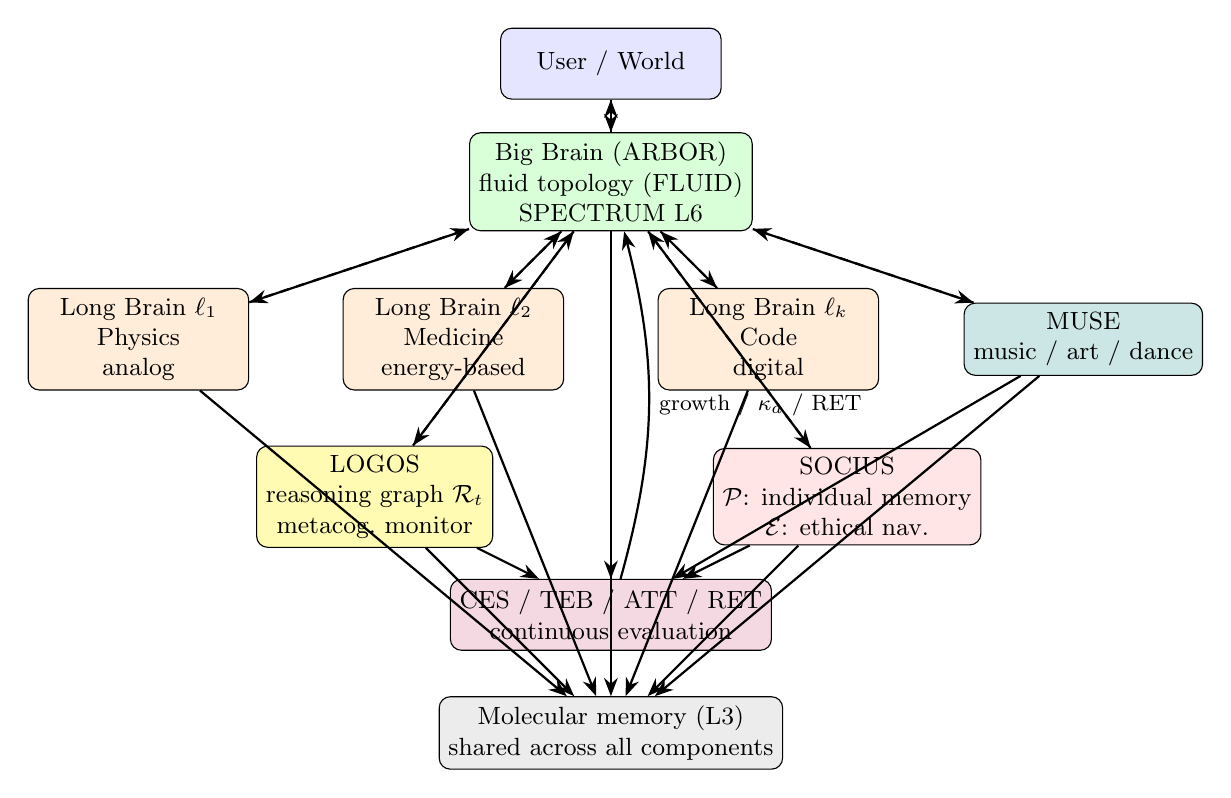
\begin{tikzpicture}[
    box/.style={rectangle, draw, rounded corners, minimum width=2.8cm, minimum height=0.9cm, align=center, font=\small},
    arrow/.style={-{Stealth}, thick}
]
\node[box, fill=blue!10]   (user)   at (0,10)   {User / World};
\node[box, fill=green!15]  (bigbr)  at (0,8.5)  {Big Brain (ARBOR)\\fluid topology (FLUID)\\SPECTRUM L6};
\node[box, fill=orange!15] (spec1)  at (-6,6.5) {Long Brain $\ell_1$\\Physics\\analog};
\node[box, fill=orange!15] (spec2)  at (-2,6.5) {Long Brain $\ell_2$\\Medicine\\energy-based};
\node[box, fill=orange!15] (spec3)  at (2,6.5)  {Long Brain $\ell_k$\\Code\\digital};
\node[box, fill=teal!20]   (muse)   at (6,6.5)  {MUSE\\music / art / dance};
\node[box, fill=yellow!30] (logos)  at (-3,4.5) {LOGOS\\reasoning graph $\mathcal{R}_t$\\metacog.\ monitor};
\node[box, fill=pink!40]   (socius) at (3,4.5)  {SOCIUS\\$\mathcal{P}$: individual memory\\$\mathcal{E}$: ethical nav.};
\node[box, fill=purple!15] (eval)   at (0,3)    {CES / TEB / ATT / RET\\continuous evaluation};
\node[box, fill=gray!15]   (memory) at (0,1.5)  {Molecular memory (L3)\\shared across all components};

\draw[arrow] (user) -- (bigbr);
\draw[arrow] (bigbr) -- (spec1);
\draw[arrow] (bigbr) -- (spec2);
\draw[arrow] (bigbr) -- (spec3);
\draw[arrow] (bigbr) -- (muse);
\draw[arrow] (bigbr) -- (logos);
\draw[arrow] (bigbr) -- (socius);
\draw[arrow, dashed] (spec1) -- (bigbr);
\draw[arrow, dashed] (spec2) -- (bigbr);
\draw[arrow, dashed] (spec3) -- (bigbr);
\draw[arrow, dashed] (muse) -- (bigbr);
\draw[arrow, dashed] (logos) -- (bigbr);
\draw[arrow, dashed] (socius) -- (bigbr);
\draw[arrow, dashed] (bigbr) -- (user);
\draw[arrow] (logos) -- (eval);
\draw[arrow] (socius) -- (eval);
\draw[arrow] (muse) -- (eval);
\draw[arrow] (bigbr) -- (eval);
\draw[arrow, bend right=15] (eval) to node[right, font=\footnotesize]{growth / $\kappa_a$ / RET} (bigbr);
\draw[arrow] (bigbr) -- (memory);
\draw[arrow] (spec1) -- (memory);
\draw[arrow] (spec2) -- (memory);
\draw[arrow] (spec3) -- (memory);
\draw[arrow] (muse) -- (memory);
\draw[arrow] (logos) -- (memory);
\draw[arrow] (socius) -- (memory);
\end{tikzpicture}
\caption{ATLAS architecture. Big Brain routes (ARBOR), adapts topology (FLUID), runs on SPECTRUM hardware. LOGOS activates on low-confidence or multi-step queries. MUSE operates via $\kappa_a$. SOCIUS maintains per-individual persistent memory ($\mathcal{P}$) and navigates ethical dilemmas via $\mathcal{E}$. CES/TEB/ATT/RET evaluates continuously. Molecular memory (L3) shared.}
\label{fig:atlas}
\end{figure}

\subsection{Emergent Properties of ATLAS}

\textbf{Self-expanding registry.} FLUID Long Brains in ARBOR can spawn sub-specialists when they encounter genuine domain gaps, autonomously registering them with the Big Brain. The registry grows without human intervention. MUSE's domain specialists ($\ell_{\text{music}}$, $\ell_{\text{visual}}$, $\ell_{\text{dance}}$) are registered in this registry and evolve as MUSE develops new aesthetic capacities.

\textbf{Substrate-native specialists.} Each Long Brain runs on the substrate that matches its domain: Physics on analog (differential equations), Medicine on energy-based (constraint satisfaction over symptoms), Code on digital (symbolic manipulation), Mathematics on quantum (proof-space search).

\textbf{TEB-driven growth.} FLUID topology adapts toward structures that improve TEB scores, grounding abstract curiosity in deployment value. Nodes and connections that consistently improve real-task efficiency are preserved; those that do not are pruned.

\textbf{Cross-specialist memory.} Molecular storage (SPECTRUM L3) is shared across all specialists. Physics Long Brain and Mathematics Long Brain share a memory substrate, enabling cross-domain retrieval without explicit routing.

\subsection{ATLAS vs.\ Prior Systems}

\begin{table}[H]
\centering\small
\begin{tabular}{lccccccc}
\toprule
\textbf{System} & \textbf{Eff.\ eval} & \textbf{Spec.\ depth} & \textbf{Opt.\ substrate} & \textbf{Fluid topo.} & \textbf{Creates} & \textbf{Deliberates}\\
\midrule
GPT-4            & No  & No  & No  & No  & No      & No \\
Gemini Ultra     & No  & No  & No  & No  & No      & No \\
Mixtral (MoE)    & No  & No  & No  & No  & No      & No \\
DeepMind AIDE    & No  & No  & No  & No  & No      & Partial \\
MuseNet/Jukebox  & No  & No  & No  & No  & Partial & No \\
o1 / o3 (OpenAI) & No  & No  & No  & No  & No      & Partial (CoT, no graph) \\
\textbf{ATLAS}   & \textbf{Yes} & \textbf{Yes} & \textbf{Yes} & \textbf{Yes} & \textbf{Yes} & \textbf{Yes} \\
\bottomrule
\end{tabular}
\caption{ATLAS satisfies all six properties. OpenAI's o1/o3 systems approximate deliberate reasoning via extended chain-of-thought but have no explicit reasoning graph, no metacognitive confidence propagation, and no consistency verifier---they remain pattern-completion systems generating chains that look like inference.}
\end{table}


%-----------------------------------------------------------
\section{Open Problems and Research Agenda}
\label{sec:open}
%-----------------------------------------------------------

The five components have different maturity levels:

\begin{table}[H]
\centering\small
\begin{tabular}{lp{3cm}p{4cm}l}
\toprule
\textbf{Component} & \textbf{Status} & \textbf{Primary open problem} & \textbf{Timeline}\\
\midrule
CES / TEB & Empirically validated ($n=4$) & Extend to full rubric tasks, larger model set & Now\\
ARBOR     & Theoretically specified & Empirical routing accuracy, depth advantage validation & 2--3 years\\
SPECTRUM  & Theoretically specified & Hardware integration of six substrates & 4--7 years\\
FLUID     & Partially validated ($n=120$ configs) & Causal memory, node creation, scale & 2--5 years\\
MUSE      & Theoretically specified & ATT validation, $\kappa_a$ calibration, embodied dance prototype & 3--6 years\\
LOGOS     & Theoretically specified & Reasoning graph benchmark, $u(c)$ calibration, OOD compositional test & 2--4 years\\
SOCIUS    & Theoretically specified & RET pilot (clinical domain), $\mathcal{P}$ persistence across sessions, ENE validation & 3--5 years\\
ATLAS     & Conceptually integrated & All of the above & 10--15 years\\
\bottomrule
\end{tabular}
\caption{Research agenda by component. Timelines assume AI-accelerated research compressing traditional estimates by 2--4$\times$.}
\end{table}

\textbf{Priority 1: ARBOR empirical validation.} Build a working ARBOR system using Llama-3.3-70B as Big Brain and fine-tuned Llama-3-8B specialists (PubMed for medicine, arXiv for physics). Measure routing accuracy and domain benchmark improvement vs.\ same-size generalist. This is executable now.

\textbf{Priority 2: FLUID at scale.} The Fluid Stability Conjecture has been empirically resolved: stable topology convergence exists within a narrow parameter band ($\theta_{\text{create}} = 0.3$, $\theta_{\text{prune}} \leq 0.01$). The next validation targets are (a) Mechanisms 2--3 (causal memory, temporal hierarchy) in isolation, (b) node creation/deletion stability as a separate open problem, and (c) scale experiments ($n_h \geq 1000$) to check whether the stable parameter band narrows at scale.

\textbf{Priority 3: SPECTRUM partial integration.} Neuromorphic + optical perception layer (L1) integrated with a digital reasoning layer (L6 transformer). Intel Loihi and silicon photonics hardware exist and are accessible. Full SPECTRUM requires quantum and molecular components not yet production-ready.

\textbf{Priority 4: LOGOS compositional benchmark.} Construct a test suite of $n=200$ problems designed to require exactly 3-, 5-, and 10-step inference chains, with each individual rule present in training but the specific combination novel. Measure accuracy of LOGOS (explicit reasoning graph) vs.\ chain-of-thought baseline (GPT-4o extended prompting). This is the first controlled test of explicit graph reasoning vs.\ elicited chain reasoning. Executable now with current software.

\textbf{Priority 5: MUSE ATT pilot.} Calibrate $\kappa_a$ weights $(\lambda_1, \lambda_2)$ on a held-out aesthetic evaluation set. Build $\ell_{\text{music}}$ specialist (fine-tuned on music theory + MIDI corpus) and test ATT Tier 1 (expert blind evaluation) on generated vs.\ human compositions. This is the first falsifiable test of the irreplaceability rebuttal. Dance requires SPECTRUM hardware; music ATT is executable with current software infrastructure.

%-----------------------------------------------------------
\section{Related Work}
\label{sec:related}
%-----------------------------------------------------------

\textbf{Evaluation.} MMLU \cite{hendrycks2021} and HumanEval \cite{chen2021} measure accuracy without compute normalization. FLOPs-per-token metrics \cite{kaplan2020} normalize by compute but not by task value. CES combines both; TEB adds deployment grounding.

\textbf{Mixture of Experts.} \cite{shazeer2017, jiang2024} route tokens to sub-networks within one model. ARBOR uses independent full-model specialists trained on domain-specific corpora---a qualitatively different form of expertise.

\textbf{Neuromorphic computing.} Intel Loihi \cite{davies2021} and IBM NorthPole \cite{ibm2023} demonstrate inference at milliwatt scale. Neither integrates with language model reasoning. SPECTRUM proposes this integration.

\textbf{Neural architecture search.} NAS \cite{zoph2017} optimizes topology before training. NEAT \cite{stanley2002} evolves topology across generations. FLUID changes topology at inference time---a fundamentally different regime.

\textbf{Open-ended learning.} Stanley et al.\ \cite{stanley2019} survey neuroevolution for open-ended capability. DeepMind's AIDE \cite{lu2024} attempts automated scientific discovery. FLUID + ARBOR provides a more complete framework for self-directed open-ended learning.

\textbf{Chain-of-thought and deliberate reasoning.} Wei et al.\ \cite{wei2022} show that eliciting intermediate steps improves accuracy on multi-step problems. OpenAI's o1/o3 extend this via extended inference-time compute. Both approaches generate text that mimics inference without enforcing logical structure: there is no explicit graph, no confidence propagation, and no consistency check. Nye et al.\ \cite{nye2021} propose ``scratchpad'' working memory but without the metacognitive monitor. LOGOS provides the formal structure these approaches approximate.

\textbf{Neurosymbolic AI.} Garcez et al.\ \cite{garcez2022} survey neural-symbolic integration. LOGOS differs: it does not translate neural representations into symbolic logic for separate processing; it layers an explicit reasoning graph on top of the neural pattern-completion substrate, activating on demand.

\textbf{Computational creativity.} MuseNet \cite{payne2019} and Jukebox \cite{dhariwal2020} generate music from prompts; DALL-E \cite{ramesh2022} and Midjourney generate images from prompts. All are reactive systems with no autonomous creative drive. Briot et al.\ \cite{briot2020} survey deep learning for music generation; none of the surveyed systems includes an aesthetic curiosity signal or cross-modal synthesis. MUSE's ATT provides the first formal evaluation criterion for creative domain replacement. Moravec's paradox \cite{moravec1988} predicts that sensorimotor and perceptual tasks (dance, embodied art) are harder to automate than abstract reasoning; MUSE addresses this through SPECTRUM's morphological substrate rather than attempting to solve it in software alone.

\textbf{Causal AI.} Pearl \cite{pearl2009} establishes the three-tier causal hierarchy. Current LLMs operate at tier 1 (observation). FLUID's causal memory enables tiers 2--3 natively.

%-----------------------------------------------------------
\section{Conclusion}
%-----------------------------------------------------------

This paper has argued that the boundary between AI and human capability is a fact about design, not a fact about nature. The argument: every claimed barrier reduces to an architectural requirement; every requirement is specifiable; every specification is satisfiable. ATLAS is the composition of seven specifications. CES/TEB measures whether the system achieves deployment value; ARBOR achieves domain depth; SPECTRUM achieves physical efficiency; FLUID achieves structural adaptability; MUSE achieves autonomous creative agency; LOGOS achieves deliberate reasoning; SOCIUS achieves relational intelligence---a persistent, evolving model of a specific person that can navigate the ethical complexity genuine care requires.

The honest status of this framework is: CES/TEB empirically validated ($\rho = 0.80$, $n=4$ models); FLUID's core stability question empirically resolved (conjecture holds conditionally, stable band identified, Lyapunov mechanism open); ARBOR, SPECTRUM, MUSE, LOGOS, and SOCIUS theoretically specified with concrete open problems and falsifiable next experiments. The contribution of this paper is the architecture of the argument---what needs to be built and in what order---not the finished system.

Five insights survive any future empirical revision:

\begin{enumerate}
    \item \textit{Language is the output, not the mind.} The transformer should be the mouth of an intelligence whose brain runs on appropriate physics.

    \item \textit{Breadth and depth are not a tradeoff.} They are a routing problem. The hospital solved this 150 years ago.

    \item \textit{Architecture is a variable.} The brain proved this. Fixed topology is an engineering convenience, not a law of intelligence.

    \item \textit{Irreplaceability is a process claim, not an output claim.} The question is not whether AI experiences music the way a human does. The question is whether the music is indistinguishable and culturally impactful. Those are falsifiable. The ATT makes them testable.

    \item \textit{Empathy is a process claim. Outcomes are the test.} The claim that AI cannot provide genuine care conflates phenomenal empathy (feeling what the patient feels) with functional empathy (producing interactions that reduce distress, build alliance, and navigate ethical complexity). RET tests the latter. The former is unfalsifiable.

    \item \textit{Saying ``therefore'' is not the same as concluding.} Current AI generates text that sounds like reasoning. LOGOS provides the structure that makes it reasoning: explicit intermediate state, confidence that propagates through chains, and a verifier that flags contradictions before they propagate. The difference between pattern completion and deliberate inference is architectural, and it is fixable.
\end{enumerate}

The people who build the systems described here have probably not yet finished high school.

\vspace{1em}
\noindent\textbf{Code and data.} CES implementation, TEB task set, scoring scripts, and CES--TEB comparison tools: \url{https://github.com/WINSTON672/lin-score}

%-----------------------------------------------------------
\begin{thebibliography}{99}

\bibitem{hendrycks2021} Hendrycks, D., et al.\ (2021). Measuring massive multitask language understanding. \textit{ICLR 2021}.

\bibitem{chen2021} Chen, M., et al.\ (2021). Evaluating large language models trained on code. \textit{arXiv:2107.03374}.

\bibitem{kaplan2020} Kaplan, J., et al.\ (2020). Scaling laws for neural language models. \textit{arXiv:2001.08361}.

\bibitem{shazeer2017} Shazeer, N., et al.\ (2017). Outrageously large neural networks: The sparsely-gated mixture-of-experts layer. \textit{ICLR 2017}.

\bibitem{jiang2024} Jiang, A.Q., et al.\ (2024). Mixtral of experts. \textit{arXiv:2401.04088}.

\bibitem{davies2021} Davies, M., et al.\ (2021). Advancing neuromorphic computing with Loihi. \textit{Proceedings of the IEEE}, 109(5), 911--934.

\bibitem{ibm2023} IBM Research (2023). NorthPole: An architecture for neural network inference with a 12nm chip. \textit{Science}, 382(6668).

\bibitem{zoph2017} Zoph, B., \& Le, Q.V.\ (2017). Neural architecture search with reinforcement learning. \textit{ICLR 2017}.

\bibitem{lin2026fluid_empirical} Lin, W.Z.\ (2026). Testing the Fluid Stability Conjecture: Empirical evidence for convergent self-structuring in dynamic neural topologies. \textit{arXiv preprint}.

\bibitem{stanley2002} Stanley, K.O., \& Miikkulainen, R.\ (2002). Evolving neural networks through augmenting topologies. \textit{Evolutionary Computation}, 10(2), 99--127.

\bibitem{bellec2018} Bellec, G., et al.\ (2018). Deep rewiring: Training very sparse deep networks. \textit{ICLR 2018}.

\bibitem{mocanu2018} Mocanu, D.C., et al.\ (2018). Scalable training of artificial neural networks with adaptive sparse connectivity inspired by network science. \textit{Nature Communications}, 9, 2383.

\bibitem{watts1998} Watts, D.J., \& Strogatz, S.H.\ (1998). Collective dynamics of small-world networks. \textit{Nature}, 393, 440--442.

\bibitem{stanley2019} Stanley, K.O., et al.\ (2019). Designing neural networks through neuroevolution. \textit{Nature Machine Intelligence}, 1, 24--35.

\bibitem{lu2024} Lu, C., et al.\ (2024). The AI scientist: Towards fully automated open-ended scientific discovery. \textit{arXiv:2408.06292}.

\bibitem{pearl2009} Pearl, J.\ (2009). \textit{Causality: Models, Reasoning, and Inference} (2nd ed.). Cambridge University Press.

\bibitem{schmidhuber2010} Schmidhuber, J.\ (2010). Formal theory of creativity, fun, and intrinsic motivation. \textit{IEEE Trans.\ Autonomous Mental Development}, 2(3), 230--247.

\bibitem{hopfield1982} Hopfield, J.J.\ (1982). Neural networks and physical systems with emergent collective computational abilities. \textit{PNAS}, 79(8), 2554--2558.

\bibitem{ramsauer2020} Ramsauer, H., et al.\ (2020). Hopfield networks is all you need. \textit{ICLR 2021}.

\bibitem{vaswani2017} Vaswani, A., et al.\ (2017). Attention is all you need. \textit{NeurIPS 2017}.

\bibitem{lewis2020} Lewis, P., et al.\ (2020). Retrieval-augmented generation for knowledge-intensive NLP tasks. \textit{NeurIPS 2020}.

\bibitem{goodman2005} Goodman, J.W.\ (2005). \textit{Introduction to Fourier Optics} (3rd ed.). Roberts \& Company.

\bibitem{sarpeshkar2010} Sarpeshkar, R.\ (2010). \textit{Ultra Low Power Bioelectronics}. Cambridge University Press.

\bibitem{hebb1949} Hebb, D.O.\ (1949). \textit{The Organization of Behavior}. Wiley \& Sons.

\bibitem{jaeger2004} Jaeger, H., \& Haas, H.\ (2004). Harnessing nonlinearity. \textit{Science}, 304(5667), 78--80.

\bibitem{payne2019} Payne, C.\ (2019). MuseNet. \textit{OpenAI Blog}.

\bibitem{dhariwal2020} Dhariwal, P., et al.\ (2020). Jukebox: A generative model for music. \textit{arXiv:2005.00341}.

\bibitem{ramesh2022} Ramesh, A., et al.\ (2022). Hierarchical text-conditional image generation with CLIP latents. \textit{arXiv:2204.06125}.

\bibitem{briot2020} Briot, J.P., Hadjeres, G., \& Pachet, F.D.\ (2020). \textit{Deep Learning Techniques for Music Generation}. Springer.

\bibitem{moravec1988} Moravec, H.\ (1988). \textit{Mind Children: The Future of Robot and Human Intelligence}. Harvard University Press.

\bibitem{wei2022} Wei, J., et al.\ (2022). Chain-of-thought prompting elicits reasoning in large language models. \textit{NeurIPS 2022}.

\bibitem{nye2021} Nye, M., et al.\ (2021). Show your work: Scratchpads for intermediate computation with language models. \textit{arXiv:2112.00114}.

\bibitem{garcez2022} Garcez, A., \& Lamb, L.C.\ (2022). Neurosymbolic AI: The 3rd wave. \textit{Artificial Intelligence Review}, 56, 12387--12406.

\bibitem{kahneman2011} Kahneman, D.\ (2011). \textit{Thinking, Fast and Slow}. Farrar, Straus and Giroux.

\bibitem{beccue2024} Beccue, M.\ (2024). 8 jobs that AI can't replace and why. \textit{TechTarget / Enterprise Strategy Group}. Retrieved from TechTarget.com.


\bibitem{horvath1989} Horvath, A.O., \& Greenberg, L.S.\ (1989). Development and validation of the Working Alliance Inventory. \textit{Journal of Counseling Psychology}, 36(2), 223--233.

\bibitem{premack1978} Premack, D., \& Woodruff, G.\ (1978). Does the chimpanzee have a theory of mind? \textit{Behavioral and Brain Sciences}, 1(4), 515--526.

\bibitem{picard1997} Picard, R.W.\ (1997). \textit{Affective Computing}. MIT Press.

\end{thebibliography}

\end{document}
